\documentclass[a4paper, 12pt]{article}

%-----------------------------------------------------
%                      PACKAGES
% ----------------------------------------------------
\usepackage[T1]{fontenc}
\usepackage[latin9]{inputenc}
\usepackage{fancyhdr}
\usepackage{geometry}
\usepackage[colorlinks=true, linkcolor=blue,citecolor=blue, urlcolor=blue]{hyperref}
\usepackage{indentfirst}
\usepackage{graphicx}
\usepackage{float}
\usepackage{setspace}
\usepackage{amsmath}
\usepackage{amssymb}
\usepackage{multirow}
\usepackage[table,xcdraw]{xcolor}
\usepackage{colortbl}
\usepackage{tabularx,booktabs}
\usepackage{enumerate}
\usepackage{titlesec}
\usepackage{caption}
\usepackage{subcaption}
\usepackage{nicefrac, xfrac}
\usepackage{subfiles}
\usepackage{mathtools}
\usepackage{bm}
\usepackage{tikz}
\usepackage[mode=buildnew]{standalone}
\usepackage{systeme}
\usepackage{stmaryrd}
\usepackage{import}
\usepackage[english]{babel} 
\usepackage{times}
\usepackage{pgfplots}
\usepackage{makecell}
\usepackage{threeparttable}
\usepackage{ragged2e}
\usepackage{tocloft}
\usepackage{booktabs}
\usepackage[acronym]{glossaries}
\usepackage{pdfpages}
\usepackage{lipsum}
\usepackage{hyphenat} 
\usepackage{xspace}
\usepackage{abntex2cite}
\usepackage{pdflscape}
\usepackage{pythonhighlight}
\usepackage{listings}
\usepackage{makecell}

%-----------------------------------------------------
%               DOCUMENT SETTINGS
% ----------------------------------------------------
\geometry{a4paper,top=30mm,bottom=20mm,left=30mm,right=20mm}

\pgfplotsset{compat=1.17} 

\numberwithin{equation}{section}
\counterwithin{figure}{section}
\counterwithin{table}{section}
% \numberwithin{lstlisting}{section}

% Defining spaces between lines
\setstretch{1.5} 

\graphicspath{{Figures/}}

\tikzset{
	font={\fontsize{11pt}{12}\selectfont}}

\setcounter{secnumdepth}{4}
\setcounter{tocdepth}{4}

% defining the height of table cells
\renewcommand{\arraystretch}{1.6}

% defining the gradient, divergence and curl operators
\newcommand{\grad}[1]{\nabla #1}
\renewcommand{\div}[1]{\nabla \cdot #1}
\newcommand{\curl}[1]{\nabla \times #1}

\def\textcite#1{\citeauthoronline{#1} \cite{#1}}
%-----------------------------------------------------
%              PRE TEXTUAL ELEMENTS
% ----------------------------------------------------
\newenvironment{epigrafe}{\newpage\mbox{}\vfill\hfill\begin{minipage}[t]{0.5\textwidth}}
{\end{minipage}\newpage}

%-----------------------------------------------------
%              PYTHON CODE SETTINGS
% ----------------------------------------------------
\definecolor{codegreen}{rgb}{0,0.6,0}
\definecolor{codegray}{rgb}{0.5,0.5,0.5}
\definecolor{codepurple}{rgb}{0.58,0,0.82}
\definecolor{backcolour}{rgb}{0.95,0.95,0.92}

\lstdefinestyle{mystyle}{
    backgroundcolor=\color{backcolour},   
    commentstyle=\color{codegreen},
    keywordstyle=\color{magenta},
    numberstyle=\tiny\color{codegray},
    stringstyle=\color{codepurple},
    basicstyle=\ttfamily\footnotesize,
    breakatwhitespace=false,         
    breaklines=true,                 
    captionpos=b,                    
    keepspaces=true,                 
    numbers=left,                    
    numbersep=5pt,                  
    showspaces=false,                
    showstringspaces=false,
    showtabs=false,                  
    tabsize=2
}

\lstset{style=mystyle}
%-----------------------------------------------------
%                     DOCUMENT 
% ----------------------------------------------------
\begin{document}
% ------- WORK INFORMATION -------
\author{Carlos Henrique Chama Puga }
\newcommand{\RA}{195416}

\title{List 2 \\ Numerical Integration}
\newcommand{\theme}{Numerical Integration}

\newcommand{\Uni}{{Universidade Estadual de Campinas}}
\newcommand{\Fac}{{Faculdade de Engenharia Civil, Arquitetura e Urbanismo}}

\newcommand{\advisor}{Porf. Dr. Philippe Devloo}
\newcommand{\coadvisor}{Dr. Giovane Avancini}

\newcommand*{\workyear}{2024}

\makeatletter

% ------- PRE TEXTUAL PAGES -------
% Could not find another way to remove the page number from the first pages
\fancypagestyle{plain}{
    \fancyhf{}% Limpa todos os campos
    \fancyfoot[C]{}%
    \renewcommand{\headrulewidth}{0pt}%
}

\pagestyle{plain}
\def\logos{
    \noindent
    \raisebox{-.5\height}{
\includegraphics[width=2.2cm]{Figures/logo-unicamp.pdf}}

    \vspace*{1.5cm}
    
    \noindent
    \begin{center} \large
        \MakeUppercase{\Uni}\\
        \Fac\\
    \end{center}
}

\def\openningpage{
  \logos
  \vskip 35mm
  \begin{center}
    \Large
      {\bf \@title}
  \end{center}
  \vskip 25mm
  \begin{flushright}
    \large
    {\textbf{Aluno:} \\ \@author - \RA}
    \vskip 10mm
    {{\bf{Docentes}}: \\
     \advisor \\
     \coadvisor}
  \end{flushright}
    \vfill
    \large
  \begin{center}
    Campinas\\\workyear
  \end{center}
}

\openningpage % Cover page

% Table of contents
\newpage
\tableofcontents 

% from here on, the page number is shown
% Chapter first page settings
\newpage
\fancypagestyle{plain}{
    \fancyhf{}% Limpa todos os campos
    \fancyhead[R]{\thepage}%
    \renewcommand{\headrulewidth}{0pt}%
}

\fancypagestyle{headings}{%
    \fancyhf{}% Limpa todos os campos
    \fancyhead[L]{\theme}% Nome do trabalho à esquerda
    \fancyhead[R]{\thepage}% Numero da página à direita
    \renewcommand{\headrulewidth}{1pt}%
}

% ------- CHAPTERS -------
\pagestyle{headings}
\section{Introdu\c{c}\~{a}o} \label{sec:intro}
A primeira lista da disciplina de M\'etodos Num\'ericos compreende uma revis\~ao de c\'alculo, abordando temas como, regra da cadeia e os  operadores gradiente, divergente e rotacional. A seguir, uma breve descri\c{c}\~ao do que foi discutido em aula.

A regra da cadeia \'e uma t\'ecnica utilizada para diferenciar fun\c{c}\~oes compostas por outras fun\c{c}\~oes. O operador gradiente, quando aplicado em uma fun\c{c}\~ao escalar, gera um vetor que aponta para a dire\c{c}\~ao de maior crescimento da fun\c{c}\~ao. O operador divergente representa a densidade volum\'etrica de fluxo que sai de um campo vetorial de um volume infinitesimal em torno de um ponto. Por fim, o operador roatcional pode ser definido como a densidade de circula\c{c}\~ao de um campo vetorial em torno de um ponto, representado pelo vetor cuja dire\c{c}\~ao e magnitude denotam o eixo e a magnitude da circula\c{c}\~ao m\'axima.

A lista foi dividida em quatro exerc\'icios, cada um abordando um dos temas supracitados. A seguir, ser\~ao apresentados os exerc\'icios e suas respectivas solu\c{c}\~oes. Real\c{c}a-se que, durante toda a realiza\c{c}\~ao dos exerc\'icios, usou-se as refer\^encias \cite{stewart2007essential} e \cite{becker1981finite} para consulta.
\section{Problem Statement}\label{sec:problem-presentation}
For this work, three different functions are chosen to be numerically integrated. These functions are presented in this section, along with their analytical solutions. To integrate the functions the Trapezoidal, the Simpson's 1/3 and 3/8, and the Gauss-Legendre rules are employed. The results obtained by these methods are compared with the analytical solutions, and the error convergence is analyzed.

For every function, one presents the function itself and the analytical solution for the integral. A code in Mathematica is developed to help with the visualization.

\subsection{Function 1}
Function 1 is represented by Eq. \eqref{eq:func1} 
\begin{equation}
    \label{eq:func1}
    f(x) = e^{-\frac{(x-1)^2}{\epsilon}} \quad \forall x \in \mathbb{R} | 0 \leq x \leq 2, \epsilon\rightarrow 0,
\end{equation}
since it depends on the parameter $\epsilon$, a simple analysis over its behaviour its made. Fig. \ref{fig:func1} shows how it is the variation of the function for differente values of $\epsilon$.
\begin{figure}[H]
    \centering
    \subfloat[$\epsilon = 10^{-1}$]{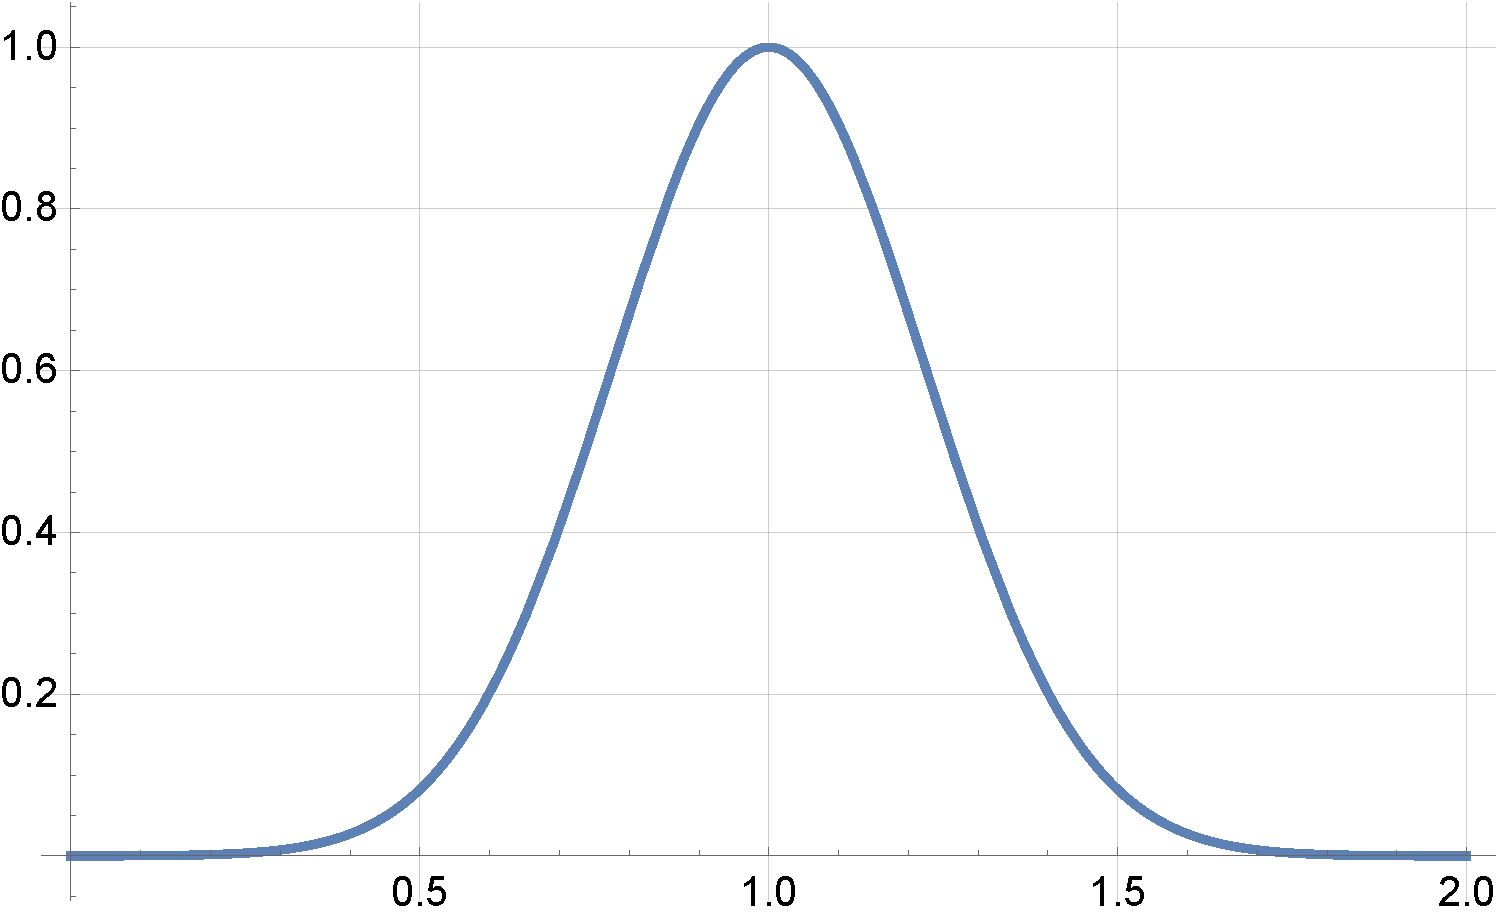
\includegraphics[width=0.5\textwidth]{../Figures/func1_e1.pdf}}\hfill
    \subfloat[$\epsilon=10^{-2}$]{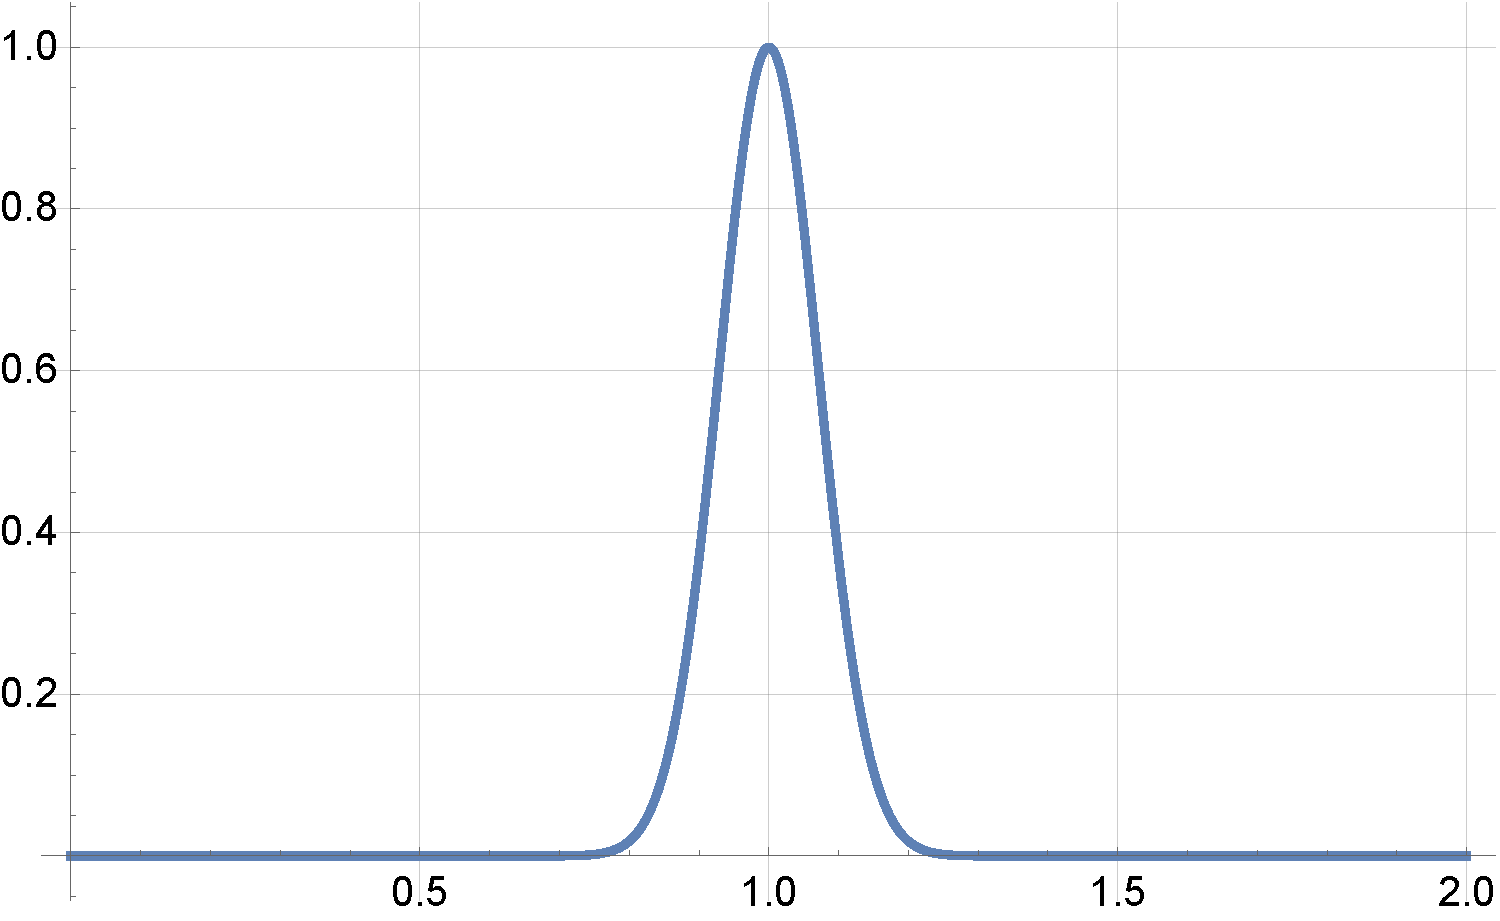
\includegraphics[width=0.5\textwidth]{../Figures/func1_e2.pdf}}\\
    \subfloat[$\epsilon=10^{-3}$]{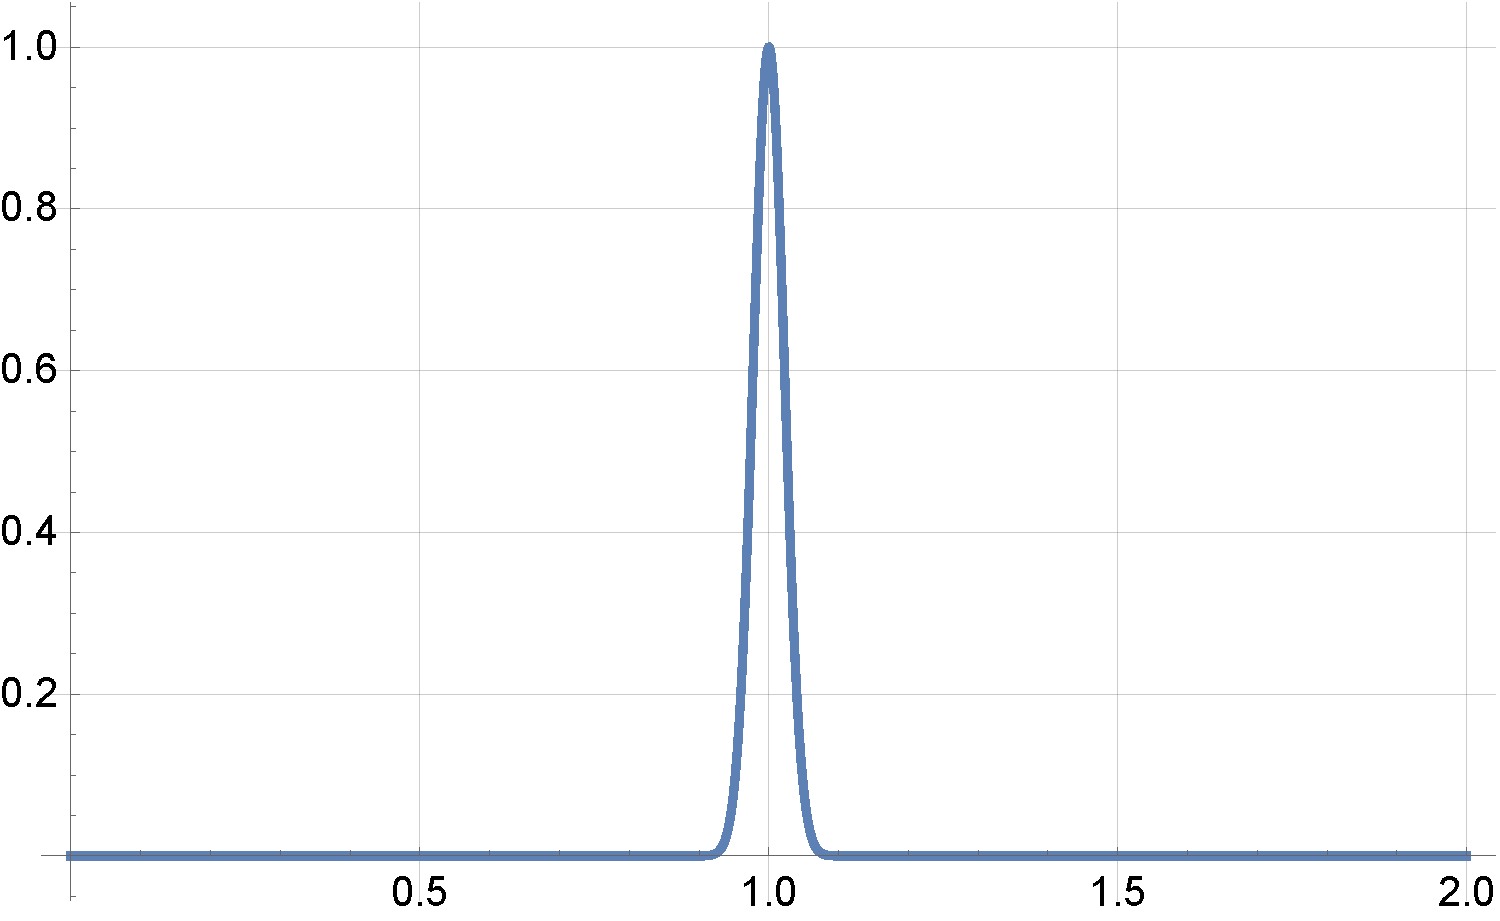
\includegraphics[width=0.5\textwidth]{../Figures/func1_e3.pdf}}\hfill
    \subfloat[$\epsilon=10^{-4}$]{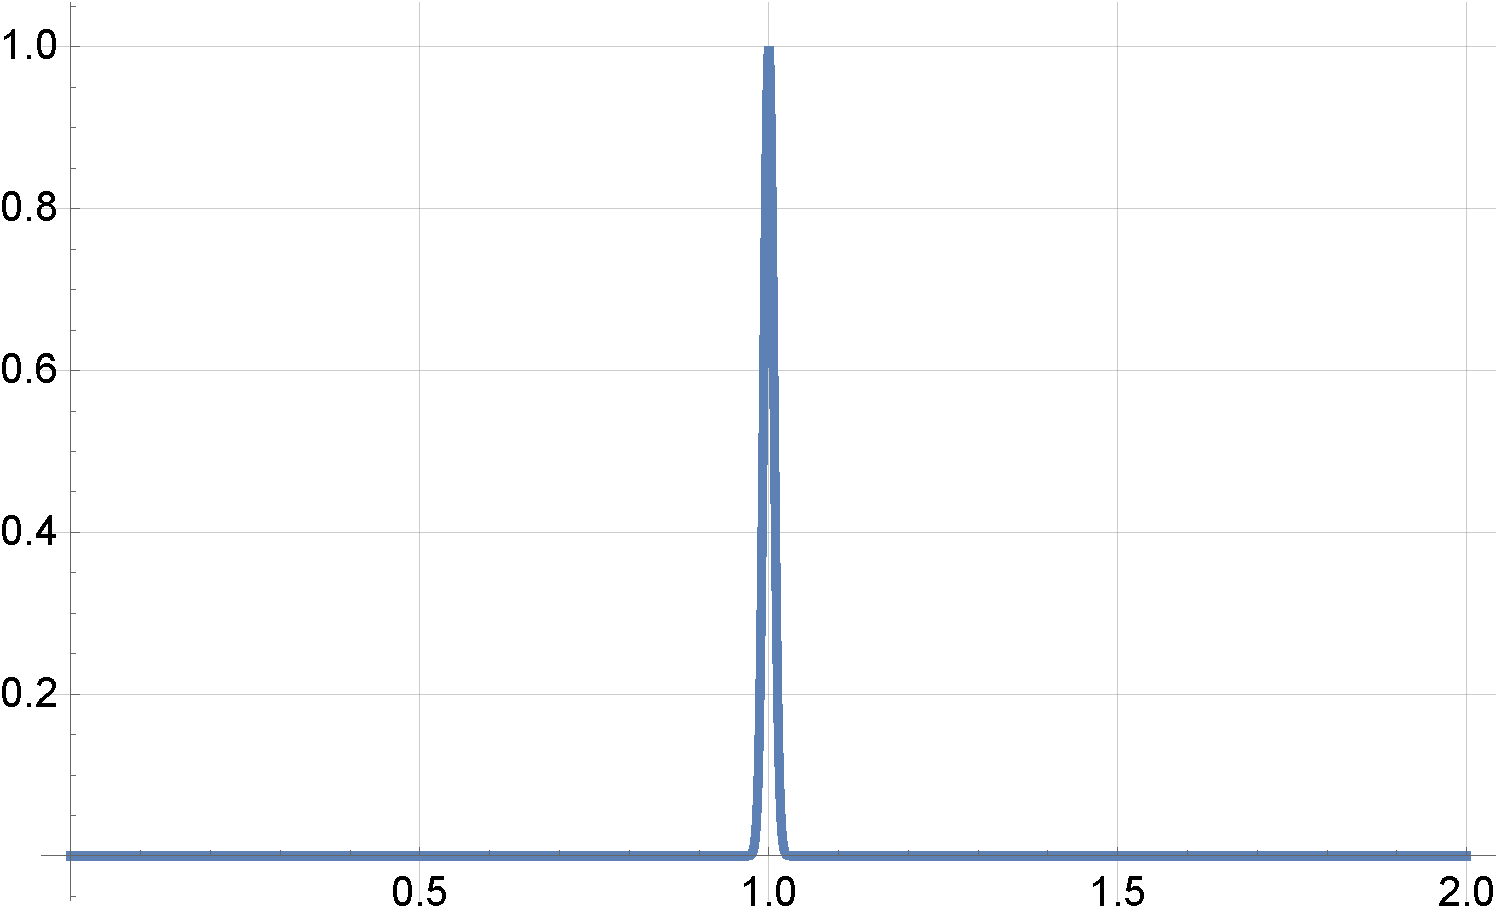
\includegraphics[width=0.5\textwidth]{../Figures/func1_e4.pdf}}
    \caption{Function 1}
    \label{fig:func1}
\end{figure}

By analyzing Fig. \ref{fig:func1}, one can note that, the lesser the value of $\epsilon$, the more the function behaves like a Dirac Delta function, which is not integrable. The analytical solution for the integral of the function is given by Eq. \eqref{eq:func1_integral}
\begin{equation}
    \label{eq:func1_integral}
    \int e^{-\frac{(x-1)^2}{\epsilon}} ~dx= \frac{\sqrt{\pi} ~\text{Erf}\left(c (- 1 + x)\right)}{2 c},
\end{equation}
in which c is a constant given by $c = pot\sqrt{10}$, and $pot$ is a integer number found in $\epsilon = 10^{-pot}$. Erf is the error function, defined by Eq. \eqref{eq:error_function}
\begin{equation}
    \label{eq:error_function}
    \text{Erf}(z) = \frac{2}{\sqrt{\pi}} \sum_{n=0}^{\infty} \frac{z}{2n + 1} \prod_{k=0}^{n} \frac{-z^2}{k}.
\end{equation}

In this work, the error function is evaluated using the Python library \texttt{scipy}.
\subsection{Function 2}
Function 2 is given by Eq. \eqref{eq:func2} and Fig. \ref{fig:func2} shows its behaviour
\begin{equation}
    \label{eq:func2}
    f(x) = x\sin\left(\frac{1}{x}\right) \quad \forall x \in \mathbb{R} | 1/100 \leq x \leq 1/10.
\end{equation}
\begin{figure}[H]
    \centering
    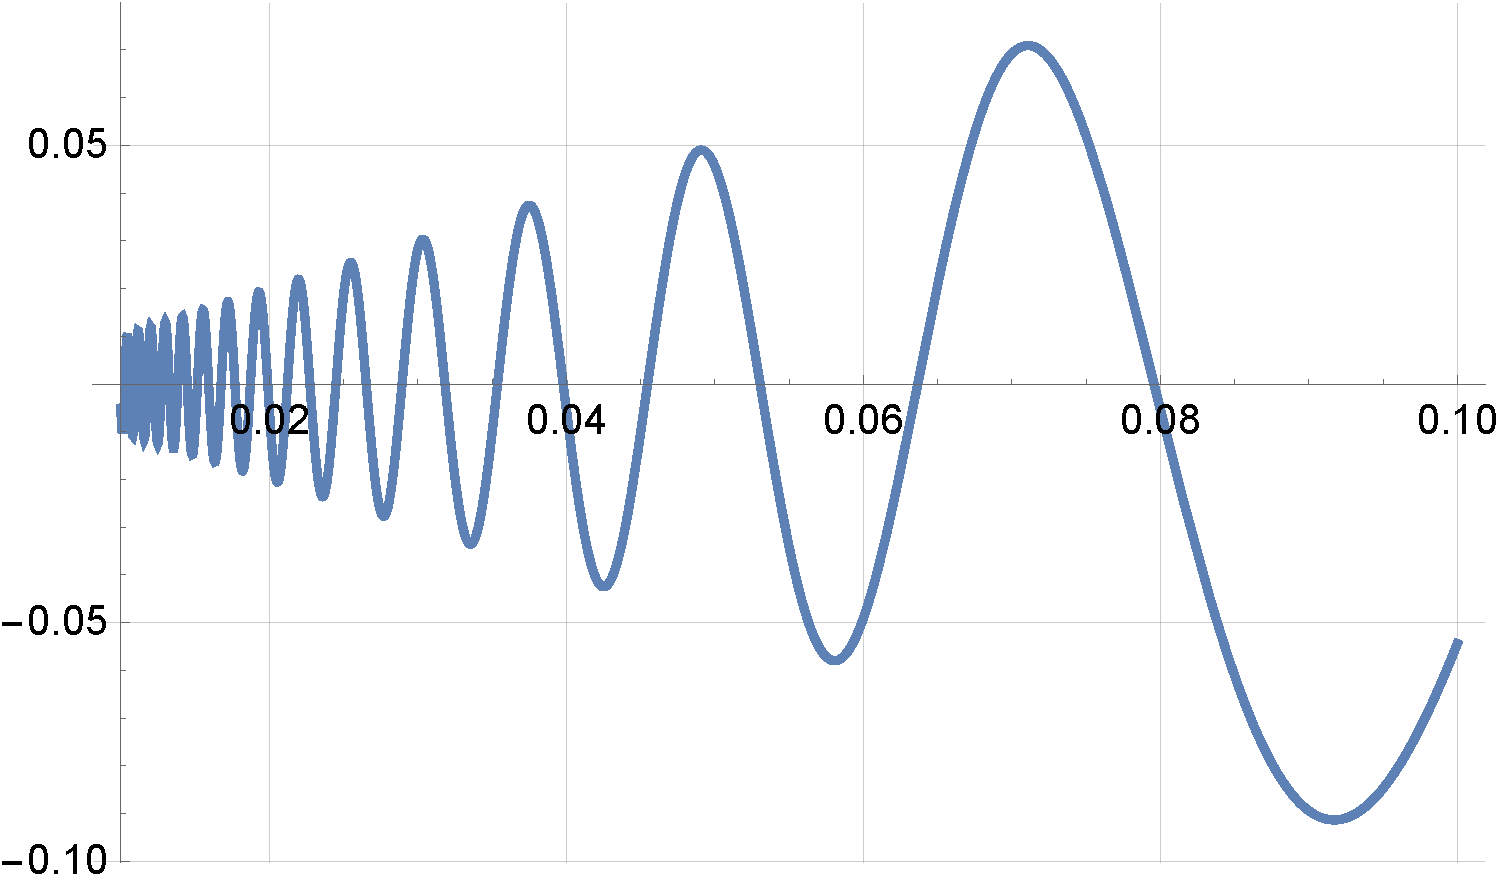
\includegraphics[width=0.5\textwidth]{../Figures/func2.pdf}
    \caption{Function 2}
    \label{fig:func2}
\end{figure}

For this function, the analytical solution for the integral is given by Eq. \eqref{eq:func2_integral}
\begin{equation}
    \label{eq:func2_integral}
    \int x\sin\left(\frac{1}{x}\right) ~dx = \frac{x}{2}\cos\left(\frac{1}{x}\right) + \frac{x^2}{2}\sin\left(\frac{1}{x}\right) + \frac{1}{2}\text{Si}\left(\frac{1}{x}\right),
\end{equation}
in which Si is the sine integral function, defined by Eq. \eqref{eq:sine_integral}
\begin{equation}
    \label{eq:sine_integral}
    \text{Si}(z) = \int_{0}^{z} \frac{\sin(t)}{t} ~dt.
\end{equation}
Eq. \eqref{eq:sine_integral} can be approximated by the Pad\'e approximants of the convergent Taylor Series, available in \href{https://en.wikipedia.org/wiki/Trigonometric_integral#Asymptotic_series_(for_large_argument)}{here}.

\subsection{Function 3}
Finally, Function 3 is given by Eq. \eqref{eq:func3} and Fig. \ref{fig:func3} shows its behaviour
\begin{equation}
    \label{eq:func3}
    f(x) = 
    \begin{cases}
        2x + 5 \quad &0 \leq x \leq 1/\pi \\
        \frac{-5\pi^2(x^2-2x-5) + 10\pi x + 2x}{1 + 5\pi^2} \quad &1/\pi \leq x \leq 2/\pi\\
        2\sin(2x) + \frac{4+20\pi^2+25\pi^3}{\pi + 5\pi^3} - 2\sin\left(\frac{4}{\pi}\right) \quad &2/\pi \leq x \leq 8/\pi
    \end{cases}.
\end{equation}
\begin{figure}[H]
    \centering
    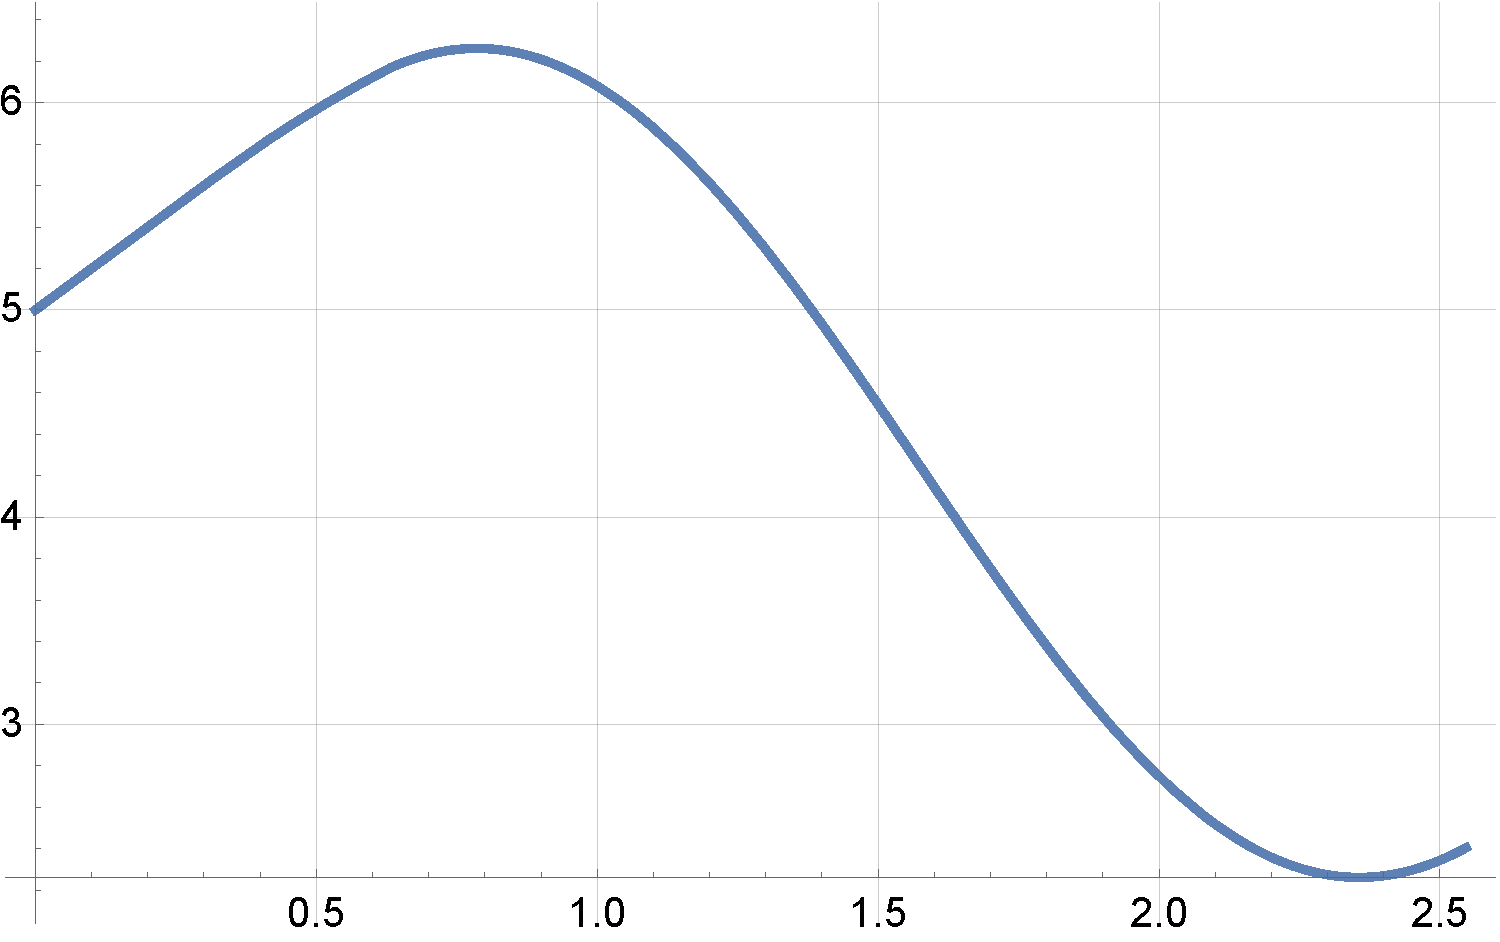
\includegraphics[width=0.5\textwidth]{../Figures/func3.pdf}
    \caption{Function 3}
    \label{fig:func3}
\end{figure}

Since the antiderivative of this function is a piecewise function, the analytical solution for the integral is given by parts as well (see Eq. \eqref{eq:func3_integral})
\begin{equation}
    \label{eq:func3_integral}
    \int f(x) ~dx = 
    \begin{cases}
        x^2 + 5x \quad &0 \leq x \leq 1/\pi \\
        \frac{25\pi^2x + x^2 + 5\pi x^2 + 5\pi^2x^2 - \frac{5\pi^2x^3}{3}}{1+5\pi^2} \quad &1/\pi \leq x \leq 2/\pi\\
        \frac{(4+20\pi^2+25\pi^3)x}{\pi + 5\pi^3} -\cos(2x) - 2x\sin\left(\frac{4}{\pi}\right) \quad &2/\pi \leq x \leq 8/\pi
    \end{cases}.
\end{equation} 
\section{Code Implementation}\label{sec:code_implementation}
This section presents the implementation of the classes used to solve the exercises proposed. For solving IVP, the RungeKutta class is developed. For BVP, the Galerkin class is implemented. Finally, for the Least Square Method, the LeastSquare class is created.

Code \ref{code:rk} shows the main function for the Runge-Kutta problem. 
\begin{lstlisting}[caption={Main function for the Runge-Kutta problem},label={code:rk},language=python]
def main_rk()->None:
    ft = lambda t, y: 1 + (t - y) ** 2
        
    rk = RungeKutta(ft, 2, 3, 0.1, 1)
    
    # 3/8 rule 4th order Runge-Kutta method
    rk.SetButcherTableau(method = "ThreeEights")
    rk.Run()

    print(rk.sol)

    rk.WriteResults("List7/Results_RK.txt")

    return
\end{lstlisting}

On line 2, the right-hand side of the differential equation is defined. On line 4, the RungeKutta object is created with the function, initial and final times, time step, and initial condition. The Butcher Tableau is set on line 7, and the Run method is called on line 8. The results are printed on line 10, and written to a file on line 12.

The main function for the Least Squares Method is shown in Code \ref{code:ls}
\begin{lstlisting}[caption={Main function for the Least Squares Method},label={code:ls},language=python]
def LeastSquareMethod()->None:
    data = [xi, yi]

    squares = LeastSquare(*zip(*data), "NonLinear")
    squares.Run()

    print(f"{squares.alpha=}")
    print(f"{squares.approx_solution=}")
    print(f"{squares.errors=}")
    print(f"{squares.total_error=}")

    return
\end{lstlisting}

Where line 2 defines the set of data points. The LeastSquare object is created on line 4, and the run method is called on line 5. The results are printed on lines 7 to 10.


\subsection{The RungeKutta Class}\label{subsec:rungekutta_class}
The RungeKutta class' attributes are displayed in Code \ref{code:rungekutta_attributes}. 
\begin{lstlisting}[caption={Attributes of the RungeKutta class},label={code:rungekutta_attributes},language=python]
@dataclass
class RungeKutta:
    ft: callable
    t0: float
    tf: float
    Dt: float
    y0: float

    ButcherTableau: list[float] = field(init=False, default_factory=list)
    c: list[float] = field(init=False, default_factory=list)
    a: list[list[float]] = field(init=False, default_factory=list)
    b: list[float] = field(init=False, default_factory=list)

    sol: list[float] = field(init=False, default_factory=list)
    step: float = field(init=False, default=0)
\end{lstlisting}

Where f\_t is the function to be solved, t0 and tf are the initial and final times, Dt is the time step, and y0 is the initial condition. The Butcher Tableau is a list of lists containing the coefficients of the Runge-Kutta method. The c, a, and b lists are the coefficients of the Butcher Tableau. The sol list stores the solution to the problem, and the step attribute is used to store the current time step.

As methods, the class has the SetButcherTableau, ConstantK, and Run. Other methods such as the EulerMethod, RK2, RK4, ThreeEightsRule, and WriteResults are also implemented. 

The SetButcherTableau method is shown in Code \ref{code:setbutchertableau_method}
\begin{lstlisting}[caption={SetButcherTableau method},label={code:setbutchertableau_method},language=python]
def SetButcherTableau(self, **var)->None:
    butcher = {"euler": self.EulerMethod(), "rk2": self.RK2(), "rk4": self.RK4(), "ThreeEights": self.ThreeEighthRule()}

    if 'method' in var:
        butcher[var['method']]

    elif 'ButcherTableau' in var:
        self.ButcherTableau = var['ButcherTableau']

    else: 
        raise ValueError("Invalid Butcher Tableau")
\end{lstlisting}

This method sets the Butcher Tableau according to the method chosen. The Euler method, Runge-Kutta 2nd order, Runge-Kutta 4th order, and Three-Eighths Rule are implemented. The user can also set the Butcher Tableau manually, by passing the desired rule. 

The ConstantK method is shown in Code \ref{code:constantk_method}
\begin{lstlisting}[caption={ConstantK method},label={code:constantk_method},language=python]
def ConstantK(self, index, t, y, k)->float:
    a = t + self.c[index] * self.Dt
    b = y + self.Dt * sum([self.a[index][j] * k[j] for j in range(index)])

    return self.ft(a, b)
\end{lstlisting}

This method is responsible for evaluating the intermediate values of the Runge-Kutta method. The index is the stage of the method, t is the current step time, y is the current value of the function, and k is the list of intermediate values. The return is the function evaluated at the intermediate point.

Finally, the Run method is shown in Code \ref{code:run_method}
\begin{lstlisting}[caption={Run method},label={code:run_method},language=python]
def Run(self)->None:
    t = self.t0
    y = self.y0

    self.c, self.a, self.b = self.ButcherTableau

    k = []
    for _ in range(self.step):
        for i in range(len(self.c)):
            k.append(self.ConstantK(i, t, y, k))

        y += self.Dt * sum([self.b[j] * k[j] for j in range(len(k))])
        t += self.Dt

        k.clear()
        self.sol.append((t, y))
\end{lstlisting}

The Run method performs the Runge-Kutta method for a given Butcher Tableau. On lines 2 and 3, the initial values of t and y are set. The Butcher Tableau coefficients (c, a, and b) are unpacked on line 5. 

From line 8 on, the method iterates over the number of steps. For each step, the intermediate values are calculated on line 10. The new value of y is calculated on line 12, and the new value of t is calculated on line 13. The intermediate values are cleared on line 15, and the t and y values are appended to the sol list on line 16.

\subsection{The Galerkin Class}\label{subsec:galerkin_class}

\subsection{The LeastSquare Class}\label{subsec:leastsquares_class}
\section{Results} \label{sec:results}
\section{Conclusion}\label{sec:conclusion}

% ------- BIBLIOGRAPHY -------
\addcontentsline{toc}{section}{References}
\bibliographystyle{abntex2-num}
\bibliography{References}

% ------- APPENDIX -------
\appendix
\section{GitHub Repository}\label{sec:github}
 The source code for this report and every code inhere mentioned can be found in the following GitHub repository: \href{https://github.com/CarlosPuga14/MetodosNumericos_2024S1}{CarlosPuga14/MetodosNumericos\_2024S1}.

\end{document}